\chapter{Transfer Learning}\label{Tl}
In this chapter, the technique of transfer learning will be introduced.
It can be considered as a large interpretation of related work.\\
This Chapter is organized as follows:    
First of all, we discuss some challenges of the traditional machine learning algorithms.
Furthermore, some real world and machine learning sample problems are discussed.\\
In the second section, the task transfer learning in the context of classification will be described.\\
There are various definitions of transfer learning in general.
Many of the solutions obtained in this chapter are made for different definitions.
Moreover, because of this the difficulty of the problem which is solved by the solutions may vary, see \ref{TlSecDef}.\\
Additionally, we will see how the difference in transfer learning is measured.\\
Furthermore, the settings of transfer learning will be introduced.
The settings implying the different setups to solve the transfer problem.\\
In the next section will introduce and explain the two main types of the transfer learning which describes the conditions of the feature space and probability distributions.
These types can be divided into approach categories.
Most of the discussed solutions are based on the formal ideas of a category.\\
The section, negative transfer deals with the problem that the provided transfer learning solutions are in fact worse than the baseline methods.
For details to kernels see section \ref{EmSubSecKernel}.

\section{Challenges of Machine Learning Algorithms}\label{TlSecChal}
The current state of 'traditional' machine learning algorithms is the assumption that training and test data existing in the same feature space and that they have the same distribution.
They are successfully learning patterns and predict events in the future.
However, it is not always possible to obtain training and test data, which matches in distribution or features space.
Reason for this may that training data, which has to be labelled, is expensive or difficult to achieve.\cite[p. 1]{Weiss.2016}\\
When it comes to supervised learning, the algorithms are designed in a way to learn from the pre-labelled data and hence it is crucial for this types of algorithms to have some.\cite[p. 6-7]{Theodoridis.2008}\\
In the 'traditional' manner, which applies to the most statistical models, to solve the problem of differences, they have to collect new training data for the new feature space or distribution of the test data and rebuild the model.\cite{Pan.2010}
Therefore, the good performance cannot be obtained, when the training and test data differs in feature space or distribution.
This is the reason, one has to find a classifier, which can be applied to the target domain, although it is trained on the source domain, which is the main motivation of Transfer Learning.\cite[p. 1.]{Weiss.2016}\\
A simple interpretation of Transfer Learning in the real world is given in the following:
Imaging two people, who want to learn piano.
One has never played any musical instrument before, while the second has previous collected knowledge on how to play music through experience with other instruments.
The latter will be able to learn the new instrument much faster than the first with no previous experience because he can transfer his general music knowledge to boost his learning of the new instrument.\cite[p. 1]{Weiss.2016}\\
When going back to machine learning, there are be more technical examples.
Consider the task of web document classification.
The goal is to classify web documents in predefined categories.
The training data in this example are university web pages, which are associated with a category by manual labelling.
If we want to classify our test data, which may not come from a university page and as a consequence the data features or distribution may be different, based on the structure or topics of the new web page.
Therefore, we can not directly apply the classifier trained on the university web page and assume a good category prediction rate on non-university web pages.
Instead, we have to collect new websites from the same type as of the test web pages, assign the category manually and finally learn a new model.
This process could be avoided if a classifier can transfer knowledge from one domain of pages into another web page domain.\cite{Pan.2010}\\
The last example is given from the topic of product reviews.
Consider the problem that a model needs to be learned, in a way that it can automatically classify positive and negative reviews on a product.
To create a source domain, one has to collect many reviews of the product and manually decide if it is positive or negative.
Then the model can be trained and can predict the sentiment of new reviews.
However, if the product changes, then the distribution of the review may change, and the traditionally learned classifier cannot be applied anymore.
Therefore, again one has to collect reviews manually and annotate them.
This can be a very expensive process, and therefore the learner should be adaptable that it can be learned on the source domain (one product category) and can help to learn the classification model (other product category).\cite{Pan.2010}

\section{Definition of Transfer Learning}\label{TlSecDef}
After more practical examples are given, the term transfer learning and associated keywords are defined in this section.\newline
In this thesis, a domain $\mathcal{D}$ is composed of a $D$-dimensional feature space $\mathcal{F}$ and a marginal probability distribution $P(\mathbf{X})$.
Formally, this means $\mathcal{D} = \{\mathcal{F},P(\mathbf{X})\}$ with $\mathbf{X} \in \mathcal{F}$.
In general, if two domains $\mathcal{X}$ and $\mathcal{Z}$ are different, then they have either different feature spaces or marginal distributions.
This can be expressed as $\mathcal{F_{Z}} \neq \mathcal{F_{X}} \vee P(x) \neq \textit{P}(z)$.\cite[. 542]{Aggarwal.2015}\\
A task $\mathcal{T}$ with a given domain D is put together with a label set $\mathcal{Y}$ and a classifier $f(\cdot)$, which is  $\mathcal{T} = \{\mathcal{Y},\textit{f}(\cdot)\}$ with $\mathbf{y} \in \mathcal{Y}$.
The function $f(\cdot)$ is a predictive function to make prediction for unseen, i.\,g. new data points $\mathbf{x}$.
From a probabilistic viewpoint we can interpret $f(x)$ as $P(y\mid x)$.
In other words given x how probable is it that label y is correctly assigned.\\
In classification, the number of varying labels will distinguish the classification problem.
The Binary classification problem for two labels, e.\,g. $\mathcal{Y} ={-1,+1}$ or discrete values, i.\,e. multiple classes, for example $\mathcal{Y}= \{1,2,..,N\}$ with $N$ classes.
In general two tasks $\mathcal{T_X}$ and $\mathcal{T_{Z}}$ are different if they have varying conditional probability distributions or label spaces, which means $\mathcal{Y_{X}} \neq \mathcal{Y_{Z}} \vee P(y\mid x) \neq P(y\mid z)$.\cite[p. 542]{Aggarwal.2015}\\ 
Note that in this thesis if we talk about transfer learning, then the training domain is denoted as $\mathcal{Z}$ and $\mathcal{X}$ represents the test domain.
For the binary case within transfer learning the following definitions are made:
Consider $\mathbf{Z} = \{(\mathbf{z}_i,y_{\mathcal{Z}_i})\}_{i=1}^{M}$ as source domain data where $\mathbf{z}_i \in \mathcal{X}_\mathcal{Z}$ as single observation and $y_{\mathcal{Z}_i} \in \mathcal{Y}_\mathcal{Z}$ is the corresponding class label, which forms the whole label vector $\mathbf{y}_\mathcal{Z}$.
Additional, the target domain data $\mathbf{X} = \{(\mathbf{x}_i,y_{\mathcal{X}_i})\}_{i=1}^{N}$.
Analogue, $\mathbf{x}_i$ is a single observation with $\mathbf{x}_i \in \mathcal{X}_\mathcal{X}$ and the corresponding class label $y_{\mathcal{X}_i} \in \mathcal{Y}_\mathcal{X}$, which is again summarized in $\mathbf{y}_\mathcal{X}$.\cite[p. 2]{Aggarwal.2015}\\
Note that we are doing the assumption here that our problem has by default more than one dimension and therefore we write a single observation as a vector of features.
The whole data is therefore represented as a matrix.
\begin{mDef}[Transfer Learning]\label{DefTl}
	Given a source domain $\mathcal{Z}$ and learning task $\mathcal{T}_\mathcal{Z}$, a target domain $\mathcal{X}$ and learning task $\mathcal{T}_\mathcal{X}$, transfer learning aims to help improve the learning of the target predictive function $f_\mathcal{X}(\cdot)$ in $\mathcal{X}$ using the knowledge in $\mathcal{Z}$ and $\mathcal{T}_\mathcal{Z}$, where $\mathcal{Z} \neq \mathcal{X}$, or $\mathcal{T}_\mathcal{Z} \neq \mathcal{T}_\mathcal{X}$.\cite[p. 542]{Aggarwal.2015}
\end{mDef}
Summarizing, our problem consist of $\mathcal{Z}=\{\mathcal{X}_\mathcal{Z},P(\mathbf{Z})\}$ and $\mathcal{T_Z}=\{\mathcal{Y_Z},f_\mathcal{Z}(\mathbf{Z})\}$ with $f_\mathcal{Z}(\mathbf{Z}) = P(\mathbf{y}_\mathcal{Z}|\mathbf{Z})$ and $f_\mathcal{X}(\mathbf{X}) = P(\mathbf{y}_\mathcal{X}|\mathbf{X})$, respectively. 
If we consider that the training and testing domain are equal and their learning tasks are the same, we step back to the traditional machine learning problem.\\
According to our challenges from section \ref{TlSecChal}, the definition can be explained with the help of the web document classification example.
The example can be divided into two cases:
In case one, if two domains are different, which means that $\mathcal{Z} \neq \mathcal{X}$ as above, then they differ in either the feature space $\mathcal{X_Z}, \neq \mathcal{X_X}$ or in their marginal probability distribution $P(\mathbf{Z}) \neq P(\mathbf{X})$.
Going back to the web document example, the first would imply that the language of the two documents is different.
The second could be caused by the fact that the documents focusing on different topics, which would be lead to different terms.\cite{Pan.2010}\\
The second case is that the tasks are different, which implies $\mathcal{T_Z} \neq \mathcal{T_X}$ and furthermore can divided into that they rather differ in the label space $\mathcal{Y_Z} \neq \mathcal{Y_X}$ or the conditional probability of the two tasks are different with $P(\mathbf{y}_\mathcal{Z}\vert \mathbf{Z}) \neq P(\mathbf{y}_\mathcal{X}\vert \mathbf{X})$.
In practice, the first would imply that the source task has only two categories, which results in a binary classification problem, although the second task has more than two labels and is, therefore, a multi-class problem.
The second case could be based on the fact that source and target documents are divided into very unbalanced user-defined classes.
Finally, if there exists a any relationship between the feature spaces of the two domains, then they are \textit{related}.\cite{Pan.2010}\\
Note that in the context of transfer learning the term \ac{DA} may appear.
Based on the discussion in \cite{Pan.2011}, the following definition can be extracted.
\begin{mDef}[Domain Adaptation]\label{DefDa}
	Given a source domain $\mathcal{Z}=\{\mathcal{X}_\mathcal{Z},P(\mathbf{Z})\}$ and learning task $\mathcal{T_Z}=\{\mathcal{Y_Z},f_\mathcal{Z}(\mathbf{Z})\}$ with $f_\mathcal{Z}(\mathbf{Z}) = P(\mathbf{y}_\mathcal{Z}|\mathbf{Z})$ and a target domain $\mathcal{X}=\{\mathcal{X}_\mathcal{X},P(\mathbf{X})\}$ and learning task $\mathcal{T_X}=\{\mathcal{Y_X},f_\mathcal{X}(\mathbf{X})\}$ with $f_\mathcal{X}(\mathbf{X}) = P(\mathbf{y}_\mathcal{X}|\mathbf{X})$. Let $\mathcal{T_Z} = \mathcal{T_X}$ and the domains $\mathcal{Z} \neq \mathcal{Z}$ in a way that $\mathcal{X}_\mathcal{Z} = \mathcal{X}_\mathcal{X}$ and $P(\mathbf{Z}) \neq P(\mathbf{X})$, domain adaptation aims to help improve the learning of the target predictive function $f_\mathcal{X}(\cdot)$ in $\mathcal{X}$ using the knowledge in $\mathcal{Z}$.
\end{mDef}
This is related to covariance shift problem.\cite{Pan.2011}
It assumes that the domain data generation is made in a way that the sampling, which the data is base on, is $P(\mathbf{y}\vert \mathbf{X})P(\mathbf{X})$.
Furthermore,  the marginal distribution $P(\mathbf{X})$ changes through the domain shift so that $P(\mathbf{X}) \neq P(\mathbf{X})$ for source domain and target domain data sampling, respectively.\cite[p. 8-9]{QuinoneroCandela.2009}\\
In practice, we can observe that the key challenge of \acl{DA} methods is to focus on aligning the differences in the marginal distribution, which can be observed in \cite{Pan.2011}, \cite{Long.}, \cite{Fernando.} and \cite{Arnold.2007}, which describe by \cite{Pan.2011} too.

\section{Measurement of Difference}\label{TlSecMeasure}
From the previous examples \ref{TlSecChal} and definitions \ref{TlSecDef}, it seems that the domains are different.
This difference needs to be determined to classify the amount of transfer which is done.
In this thesis, it is measured with the \ac{MMD} and \ac{KLD}.
Note that they only consider the differences in the marginal domain distributions.
Another, point worth to mention is that the methods, which we will introduce later on, are based on these measures.
For example the \acl{TCA} and the \acl{JDA} solutions are using the \acs{MMD} in the optimization problem.
On the other hand, the authors of TrAdaBoost using the \acs{KLD} to determine the difference in domains, to measure the quality of the transfer-algorithm.

\subsection{Maximum Mean Discrepancy}\label{TlSubSecMMD}
First, the \acl{MMD} is a non-parametric function to measure the difference of two \ac{IID} samples $\mathbf{X}$ and $\mathbf{Y}$ drawn from p and q respectively introduced by \cite[p. 724-728]{Gretton.2012}.
Two samples of a random variable are independent, if a current sample is not influenced by any previous samples and will not influence following samples.
Identically  distributed, as the name says, requires that the random variables having the same distribution.\cite[p. 7-8]{Czado.2011}\\
The \acs{MMD} is based on samples drawn from two distributions.
It measures the distance between the expectations of two samples, $\textbf{X}=\{x_1,...x_M\}$ and $\textbf{Y}=\{y_1,...y_M\}$
in a \ac{RKHS} $\mathcal{H}$.
Assuming that $\mathbf{X} \sim p$ and $\mathbf{Y} \sim q$.
Furthermore, if $\mathcal{H}$ is a Hilbert space, then the mapping function is defined as $f(x) = \langle f,\phi(x) \rangle_\mathcal{H}$ with $\phi(x) = k(x,\cdot)$ as positive semi-definite kernel.
Note that a \ac{PSD} kernel, has only non negative eigenvalues.\cite[p. 30]{Scholkopf.2001}
Finally, the \acs{MMD} and his empirical estimation is defined as \eqref{EqMMdExp} and \eqref{EqMMdExpEm}:\cite[p. 726-727]{Gretton.2012}
\begin{equation}\label{EqMMdExp}
MMD[\mathcal{F},p,q]^2:=\big[sup_{\|f\|_\mathcal{H} \le 1 }(E_{x\sim p}[f(x)] - E_{y\sim q}[f(y)])\big]^2
\end{equation}
\begin{equation}\label{EqMMdExpEm}
MMD_e[X,Y]:= \abs{\frac{1}{M}\sum_{i=1}^{M}f(x_i) - \frac{1}{N}\sum_{i=1}^{M}f(y_i)}_{\mathcal{H}}
\end{equation}
Where $f:\mathcal{X} \to \mathbb{R}$ is a member of the function class $\mathcal{F}$.\\ This means that considering the \acs{RKHS} $f(x)$ and $f(y)$ are based on the same $\phi(\cdot)$, i.\,e. kernel function for any $\mathbf{x,y} \in \mathbb{R}$.\cite[p. 36]{Scholkopf.2001}\\
Note that the empirical \acs{MMD} is biased.
If p and q both are equal probability distributions, respectively $p = q$, then the \ac{MMD}\textsubscript{e} = 0.\cite[p. 726-727]{Gretton.2012}\\
The \acs{MMD} is symmetric after it takes the absolute value, as shown in \eqref{EqMMdExpEm}.\\
Another advantage of \eqref{EqMMdExpEm} is that it can be calculated based on samples.
Unlike the following Kullback-Leibler Divergence where the density has to be estimated before, the \acs{KLD} can be calculated.\cite{Long.2015}\\
The code for the \acs{MMD} estimation can be obtained from the website of Gatsby Computational Neuroscience Unit\footnote{\url{http://www.gatsby.ucl.ac.uk/~gretton/mmd/mmd.htm}}, which uses the standard Gaussian kernel for feature mapping.

\subsection{Kullback-Leibler Divergence}\label{TlSubSecKLD}
The \acl{KLD} is also named Kullback-Leibler-Risk.
It needs two probability distributions f and g of a random Variable X.
For discrete variables $x_i, i=1,..,m$ with $p_i=f(x_i)$ and $q_i=g(x_i)$ as probabilities, respectively the \acs{KLD} is calculated as:
\begin{equation}
KL(g\mid f) = \sum_{i=1}^{m}p_i\log\frac{p_i}{q_i}
\end{equation} 
For continues variables the \ac{KLD} is computed:
\begin{equation}
KL(g\mid f) = \int f(x)log\frac{f(x)}{g(x)} dx
\end{equation}
For all f and g it is $KL(g\mid f) \ge 0$. Next $KL(f\mid f) = 0$ and finally, if $KL(g\mid f) = 0$, then $f = g$, which implies that the two distribution are nearly the same.
Note that the \acs{KLD} is not symmetric and as a consequence the  \cite[p.5-7]{Commenges.}\\
Because the density has to be estimated, the \acs{KLD} in this thesis will be determined by a Bayesian method approach, which is described in the supplementary material of \cite{Berkes.2011}.
The source code for the \acs{KLD} estimation can be found at GitHub\footnote{\url{https://github.com/pberkes/neuro-kl}}.

\section{Settings of Transfer Learning}\label{DefTlSecSett} %
In this section, the different settings of transfer learning are proposed.
There are various settings of the transfer learning definition, which specifies the composition of domains and tasks and how they are related to each other.
Therefore, each setting has his requirements on how labelled data in the source and target domain is available.
In general, the settings could be summarized with 'What to transfer?' and 'How to transfer?'.
The various settings are related to some traditional machine learning task.\cite{Pan.2010}\\
As we will see in the following, the definitions of homogeneous (\ref{TlSecHomo}) and heterogeneous (\ref{TlSecHetero}) transfer learning and the definitions of the settings will overlap.\cite[p. 5-6]{Weiss.2016}\\
In general, we will stick to the definitions of homogeneous and heterogeneous, because these are more general in comparison with the settings.
Therefore, the settings are used to formulate the categories of the transfer learning methods more precisely.
Additionally, but more importantly, we want to focus on the fact, whether labelled or unlabeled target data are required for the knowledge transfer.
The methods will be explained within the section of homogeneous and heterogeneous transfer learning.
The relationship is shown in figure \ref{FigSettingsTransferLearning}.
\begin{figure}
	\centering
	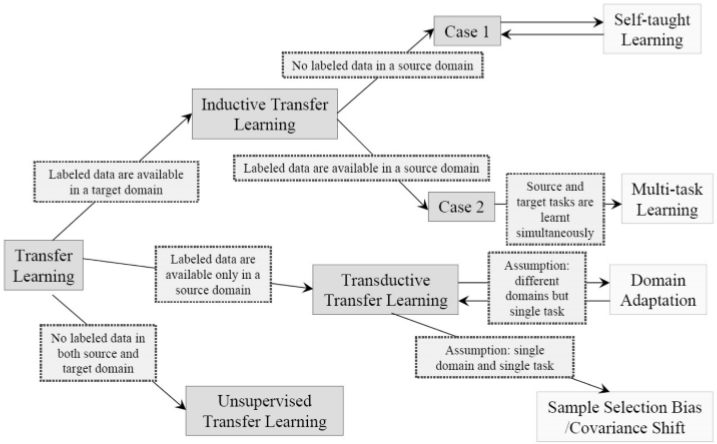
\includegraphics[width=.8\linewidth]{figures/SettingsTransferLearning.png}
	\caption[Settings of Transfer Learning]{The various settings of transfer learning approaches and there relation to traditional machine learning problems.\cite{Pan.2010}}
	\label{FigSettingsTransferLearning}
\end{figure}

\subsection{Inductive Transfer Learning}\label{TlSubSecInduc}
The setting \ac{ITL} takes the assumption that the target task and the source task are different regardless of whether the source and target domains are different or not.
Methods of this setting requiring some labelled test data to \textit{induce} a predictive model $f_\mathcal{X}(\mathbf{X})$ for the training domain.\cite{Pan.2010}
Therefore Pan et al. formulated the following definitions.
\begin{mDef}[Inductive Transfer learning {\cite{Pan.2010}}]\label{DefITL}
	 Given a source domain $\mathcal{Z}$ and a learning task $\mathcal{T_Z}$, a target domain $\mathcal{X}$ and a learning task $\mathcal{T_X}$, inductive transfer learning aims to help improve the learning of the target predictive function $f_\mathcal{X}(\cdot)$ in $\mathcal{X}$ using the knowledge in $\mathcal{Z}$ and $\mathcal{T_Z}$, where $\mathcal{T_Z} \neq \mathcal{T_X}$, while some labeled target domain data is available.
\end{mDef} 
With this in mind, there are in fact two special cases to consider.
The first one tries to achieve high performance in the target task by requiring not only some labelled test data but lots of labelled training data.
This is related to the multi-task learning approach where a learner tries to learn both domains, the source and target domain simultaneously.\cite{Pan.2010}\\
In the second case, there are no labelled source data at all available.
The goal is similar to the self-thought learning setting.
The challenge of self-thought learning is information from the source domain can not be applied to the target because they are not the same and therefore can not be used directly.
Summarizing, because the source data can not be used directly, we have to find are parts of the data which can be combined with a few labelled target data to reach the goal.\cite{Pan.2010}\\
In the section \ref{TlSubSecInstance}, we will give an example of an instance based approach, based on the inductive transfer learning setting.
Note that this solution tries to aligning the marginal distributions with some labelled data, which is little different to the original definition of inductive learning.

\subsection{Transductive Transfer Learning}\label{TlSubSecTrans}
The \ac{TTL} setting assumes that the tasks of the two domains are the same, but the source and target domains are different.
Furthermore, it requires a lot of labelled data in the source domain and assumes no labelled data in the target domain and has the requirement that some target data is available at training time.\cite{Pan.2010}
The formal definition is made with:
\begin{mDef}[Transductive Transfer Learning {\cite{Pan.2010}}]\label{DefTTL}
	 Given a source domain $\mathcal{Z}$ and a corresponding learning task $\mathcal{T_Z}$, a target domain $\mathcal{X}$ and a corresponding learning task $\mathcal{T_X}$, transductive transfer learning aims to improve the learning of the target predictive function $f_\mathcal{X}(\cdot)$ using the knowledge in $\mathcal{Z}$ and $\mathcal{T_Z}$, where $\mathcal{Z} \neq \mathcal{X}$ and $\mathcal{T_Z} = \mathcal{T_X}$.In addition, some unlabeled target domain data must be available at training time.
\end{mDef}
The term \textit{transductive} has several meanings.
In traditional machine learning, it means that \underline{all} target domain data has to be available at training time and as a consequence, the learned model cannot be reused with new, i.\,e. unseen data.
However, this can be relaxed, which the result that in the transfer learning topic \textit{transductive} means that the task must be the same and only \textit{some} unlabeled target has to be available at training time.\cite{Pan.2010}\\
The transductive setting can be divided into two special cases:
The feature spaces between the source and target data are different with $\mathcal{Z} \neq \mathcal{X}$.
This is related to the definition of heterogeneous transfer learning from \ref{TlSecHetero}.
The second case is that the feature spaces are the same, but the marginal probability distributions differ, i.\,e. $P(\mathbf{Z}) \neq P(\mathbf{X})$.\cite{Pan.2010}\\
In this case, the transductive transfer learning is related to the domain adaptation task from \ref{DefDa}.
An example of transductive transfer learning method is given in \cite{Wang.2008}.
In this, they cluster the unlabeled target data for pseudo label generation and using a custom dimension reduction with the clustered target data and the labelled source data to create a subspace.
Summarizing, because the two domains are different, transductive transfer learning aims to improve the learning by using the source data and task in combination with a few unlabeled target data.

\subsection{Unsupervised Transfer Learning}\label{TlSubSecUnsuper}
The last one, the unsupervised transfer learning section, which is obvious not part of the category supervised learning, but will be described for completeness.
It assumes that in both domains no labeled data is available.
Furthermore, the task of the source and target data are different.
In comparison with the supervised learning transfer learning methods, the goal is not to find labels for the target data but solving clustering, dimensionally reduction and density estimation.\cite{Pan.2010}
Finally, we can give the following definition.
\begin{mDef}[Unsupervised Transfer Learning {\cite{Pan.2010}}]\label{DefUTL}
	 Given a source domain $\mathcal{Z}$ with a learning task $\mathcal{T_Z}$, a target domain $\mathcal{X}$ and a corresponding learning task $\mathcal{T_X}$, unsupervised transfer learning aims to help improve the learning of the target predictive function $f_\mathcal{X}(\cdot)$ in $\mathcal{X}$ using the knowledge in $\mathcal{Z}$ and $\mathcal{T_Z}$, where $\mathcal{T_Z} \neq \mathcal{T_X}$ and $\mathcal{Y_Z}$ and $\mathcal{Y_X}$ are not observable.
\end{mDef}
Note that the predictive function $f_\mathcal{X}(\cdot)$ aims for example to find the cluster centres.
An example for Unsupervised transfer learning methods can be given from section \ref{TlSubSecHomoSymFeature} when the corresponding learner will be replaced with an unsupervised learning algorithm.
Examples are discussed in section \ref{TlSubSecHomoSymFeature}.
Summarizing, this setting aims to improve the respective tasks by the use of the source data or task.
This is, in fact, similar to the inductive transfer learning setting from section \ref{TlSubSecInduc}.\cite{Pan.2010}

\section{Homogeneous Transfer Learning}\label{TlSecHomo}
In this section, the homogeneous transfer learning approach will be introduced.
In general, it has the assumption that the feature spaces are equal and the conditional or marginal distributions of the domains are different.
There are three main goals of homogeneous transfer learning.
The first is one is to align the marginal distribution difference.
The second is to correct the difference in the conditional probability distributions, and the last one tries to align both, the marginal and conditional distribution difference.\cite[p. 6]{Weiss.2016}
This is formalised in the same way as the previous definition, which is influenced by the formulation of Pan et al. from \cite{Pan.2010}.
\begin{mDef}[Homogeneous Transfer Learning]\label{DefHomogeneous}
	Given a source domain $\mathcal{Z}$ and learning task $\mathcal{T_Z}$, a target domain $\mathcal{X}$ and learning task $\mathcal{T_T}$, homogeneous transfer learning aims to help improve the learning of the target predictive function $f_\mathcal{T}(\cdot)$ in $\mathcal{X}$ using the knowledge in $\mathcal{Z}$ and $\mathcal{T_Z}$, where $\mathcal{X_Z} = \mathcal{X_X}$ and $\mathcal{Y_Z} =\mathcal{Y_X} $, but $P(\mathbf{Z}) \neq P(\mathbf{X})$ and/or $P(\mathbf{y_\mathcal{Z}}\vert \mathbf{Z}) \neq P(\mathbf{y_\mathcal{X}}\vert \mathbf{X})$.\cite[p. 4]{Weiss.2016}
\end{mDef}
If the differences only exit in the marginal distribution, then we can build another relation to \acl{DA} from definition \ref{DefDa}.
Refer to section \ref{TlSecChal}, for examples on why the distribution can be different.\cite[p. 6-7]{Weiss.2016}\\ 
The homogeneous transfer learning category can be split up in five general approaches:
Instance-transfer, symmetric-feature transfer, asymmetric-feature transfer, parameter transfer and relational-knowledge transfer.
These approaches are sometimes called categories of information transfer.
They give a general understanding of how the methods are trying to align the differences.\cite[p. 6-7]{Weiss.2016}
Unlike the previous definitions, settings and explanations, which describing the problem and only giving an abstract solution with the predictive function.
\subsection{Instance-transfer}\label{TlSubSecInstance}
The instance transfer method tries to full fill the goal of aligning the marginal distribution by reweighting some source data.
This reweighted data is then directly used with target data for training.
It seems that these type of algorithm works best when the conditional probability is the same in source and target domain \cite[p. 6]{Weiss.2016}\\
In the following, we will present such an Instance transfer algorithm.
The so-called \textit{TrAdaBoost} which is proposed by Dai et al.\cite{Pan.2010}\\
\subsubsection{TrAdaBoost}
The TrAdaBoost\footnote{\url{https://github.com/LinZhineng/transfer-learning/tree/master/tradaboost}} algorithm extends the boosting-based learning algorithm.
The Algorithm follows the instance transfer definition and assumes that the marginal probability distribution are different, but the conditional probability distribution are the same.\cite{Dai.}
It is originally proposed as two class solution, but there are extension like MsTrAdaBoost for multi-class problems.\cite{Huang.2012}\\
The main goal is to reuse some source data in the target domain.
The source data is in general considered as out-dated.
It uses a small amount of labelled target data, considered as new data, which is called same-distribution training data.
Therefore, and because of definition \ref{DefITL}, the method has an inductive setting.
This new data is then used to help to vote on the usefulness of the old training data.\cite{Dai.}\\
The voting filters via the boosting approach.
It boosts the part of the data which is not too far away from the same-distribution training data.
The part of the source data, which is outvoted and therefore has a different distribution is together with the near data is called diff-distribution training data.
The voted part of the data is used to make the knowledge transfer.
Furthermore, the same-distribution training data and the diff-distribution training data are forming the new source data for the training.
In the corresponding article, the weighted-\acs{SVM} is used as the underlying learner.
It is rather crucial that the learner has some weighting function because the filtering is done with weighting.\cite{Dai.}\\
The TrAdaBoost algorithm has two free parameters, which is the number of iterations and the initial value of the weight vector.
Suppose the number of fixed iterations is $T$ and the unlabeled target dataset $\mathbf{X}$.
Consider $\mathbf{Z}_D$ as diff-distribution training dataset with labels of size $N$ and the same-distribution data (from the target data) with labels $\mathbf{Z}_S$ has $M$ points.
This forms the complete training set $\mathbf{Z}=\mathbf{Z}_D\cup \mathbf{Z}_S$, with $N+M$ entries, with $\mathbf{\mathbf{Z}}=\{(\mathbf{z}_i,y_i))\}$, where $y_i$ is the label for the ith-data point with $y\in {0,1}$ and $x_i$ with \cite{Dai.}:
\begin{equation*}
	\mathbf{z}_i = \begin{dcases}
						\mathbf{z}_i^D, \>\>\>\> i = 1,\dots,N\\
						\mathbf{z}_i^S, \>\>\>\> i = N +1,\dots,N+M
			  	   \end{dcases}
\end{equation*}
In every iteration, the learner is trained with this training set and predicts for the training $\mathbf{Z}$, and the unlabeled target dataset $\mathbf{X}$.
The prediction in this context is called a hypothesis.
In this article, the training loss is defined as the difference between the training data prediction and the ground truth label.
Furthermore, the prediction error is the difference between the ground truth target labels and the prediction.
Note that the label for $\mathbf{Z}_S$ is predicted, too.\cite{Dai.}\\
At this point the filtering takes place.
If a diff-distribution data point is mistakenly predicted, then it may be caused by the difference of this instance to the same-distribution training data.
When this is the case, the \textit{TrAdaBoost} algorithm reduces the weight for this data point, and therefore this point will affect the learning process less than in the current iteration.
This is done via updating the weight vector $\mathbf{w}^t=\{w_1^t,\dots,w_{N+M}^t\}$ in the $t$-th iteration with \cite{Dai.}:
\begin{equation}\label{EqTrAdaWeighting}
	w_i^t+1=\begin{dcases}
				w_i^t\beta^{\vert h_t(\mathbf{z}_i )-y_i\vert}, \>\>\>\>\>\> 1\le i \le N \\
				w_i^t\beta_t^{-\vert h_t(\mathbf{z}_i )-y_i\vert}, \>\>\> N+1\le i \le N+M
			 \end{dcases}
\end{equation}
Where $ h_t(\mathbf{x}_i )$ is the predicted label for the $i$-th data point.
Furthermore, the different betas are set to $\beta_t = \epsilon_t / (1-\epsilon_t)$, where $\epsilon_t$ is a weighted error function and $\beta= 1 / 1 + \sqrt{2\ln n/T}$.
Note that $\epsilon_t$ function value is required to be less than 0.5.\\
In equation \eqref{EqTrAdaWeighting} can be seen that the same distribution training data uses another weighting function instead of the weighting function for the diff-distribution training data.
This causes that the weight gain for the target data can be much higher as for the source data.\\
The $\beta$, which is multiplied with the weight for the training data, is bound by $\beta^{\vert h_t(\mathbf{x}_i )-y_i\vert} \in (0,1]$.
After the $T$ iteration, the algorithm creates the final hypothesis of the labels based on the previous iterations.
Note that only steps which are in the range of $\{\lceil T /2 \rceil,\dots,T\}$ are considered.\cite{Dai.}\\
We proceed by describing some theoretical ideas of the \textit{TrAdaBoost}, which is claimed to be theoretical similar to the underlying \textit{AdaBoost}.
The convergence rate of the algorithm over the diff-distribution training data $\mathbf{Z}_D$ can be bound by $\mathcal{O}\big(\sqrt{\ln N /T }\big)$
With an increasing number of iterations, the error rate can be minimized.
Furthermore, the error rate of the same-distribution data for the final hypothesis (final label assignment based on the T iterations) can be upper bounded with.
\begin{equation}
	\epsilon \le 2^{\lceil T / 2\rceil} \prod_{t=\lceil T / 2\rceil}^{T} \sqrt{\epsilon_t(1-\epsilon_t)}
\end{equation}
At this point, the required $\epsilon_t < 0.5$ becomes important.
If so, then the final hypothesis will be increasingly smaller after each iteration.\cite{Dai.}

\subsection{Symmetric-Feature-Transfer}\label{TlSubSecHomoSymFeature}
The solutions, which implementing the symmetric feature transfer are trying to find a common latent subspace for source and target domain, with the goal to reduce the marginal distribution differences.
In the subspace, they should preserve the underlying structure of the data, which can be any relation in between the data.
An example of a symmetric feature space transfer method is \ac{TCA}, which will be discussed in the following.\cite[p. 6]{Weiss.2016}
\subsubsection{Transfer Component Analysis}
The \acs{TCA} method is presented by Pan et al. in \cite{Pan.2011}\footnote{\url{https://github.com/LinZhineng/transfer-learning/tree/master/tca}}.
The authors proposed \acs{TCA} to support classifier for unsupervised and semi-supervised learning.\cite{Pan.2011}
However, the resulting kernel and the transformation matrix can be used to train a kernel based learner like the \acs{SVM}, which is in fact supervised.
It has the assumption, which makes it a homogeneous transfer method that the conditional distribution is the same, i.\,e. $ P(\mathbf{y}_\mathcal{Z}\vert \mathbf{Z}) = P(\mathbf{y}_\mathcal{X}\vert \mathbf{X})$, but the marginal probability distribution are different.
Furthermore they assume that there exists a feature transformation $\phi$, which can align the differences, i.\,e. $P(\phi(\mathbf{Z})) \approx(\phi(\mathbf{X}))$ and preserve $P(\mathbf{y}_\mathcal{Z}\vert \phi(\mathbf{Z}))\approx P(\mathbf{y}_\mathcal{X}\vert \phi(\mathbf{X}))$.\cite{Pan.2011}\\
Additionally, we will see that \acs{TCA} requires target data in the training process and is therefore transductive.\\
In general there may exits underlying data structures and relationships in between them.
Some of them do cause the distribution difference, and some of them are the reason for relations between the source and target domain.
The part of the data which causes the relation is called \textit{transfer component} and should be found to preserve structure but at the same time aligning the differences.\cite{Pan.2011}\\
Pan et al. are using their previous work from \cite{Pan.2008}.
In this they have presented the \ac{MMDE}, which is an extension of the \acs{MMD} metric defined in section \ref{TlSubSecMMD}.
It states that finding a transformation which minimizes the \acs{MMDE}, then transformation will draw the marginal distribution closer together.\\
Consider $\mathbf{K}$ as a cross-domain kernel, as a composition of the source and target domain, in the embedded subspace which has the form:\cite{Pan.2011}
\begin{equation}\label{EqTCAKernel}
\mathbf{K} = 
	\begin{bmatrix}
	K_{\mathcal{Z}}\>\>\>\> K_{\mathcal{ZX}} \\
	K_{\mathcal{XZ}}\>\>\>\> K_{\mathcal{XX}}
	\end{bmatrix}
\end{equation}
Where $\mathbf{K} \in \mathbb{R}$ with size $N\times N = (N_\mathcal{Z} + N_\mathcal{X}) \times (N_\mathcal{Z}+ N_\mathcal{X})$.
This is the kernel over all data points and should be learned in a way that the marginal distribution in the subspace is aligned and the data variance (preserve data structure) is maximized.
For that the \acs{MMD} from section \ref{TlSubSecMMD} is rewritten as $tr(\mathbf{KM})$.
Where $\mathbf{M}$ is the \acs{MMD} matrix as:\cite{Pan.2011}
\begin{equation}\label{EqTCAMMD}
(M)_{ij}= \begin{dcases}
\frac{1}{N_\mathcal{Z}^2},\>\>\> \mathbf{x_i},\mathbf{x_j} \in \mathcal{Z}\\
\frac{1}{N_\mathcal{X}^2},\>\>\> \mathbf{x_i},\mathbf{x_j} \in \mathcal{X}\\
\frac{-1}{N_\mathcal{Z}N_\mathcal{X}},\>\>\> otherwise
\end{dcases}
\end{equation}
This is, in fact, the same transformation matrix for integrating \acs{MMD} as it is done by an asymmetric approach described in section \ref{TlSubSecHomoAsymFeature}.
The objective function of the \acs{TCA}, uses the \acl{MMDE}, which results in the following equation:\cite{Pan.2011}
\begin{equation}\label{EqTCAMMDEObjt}
	\max_{\mathbf{K}\succeq 0} tr(\mathbf{KM}) - \lambda tr(\mathbf{K})
\end{equation}
With this, the \acs{MMDE} is simply the extensions of the \ac{MMD} with a regularization term, which can be seen on the right side of equation \eqref{EqTCAMMDEObjt}.\cite{Pan.2011}\\
In this objective, if the first term is minimized, then the aligning happens.
Furthermore, if the second term, which is the constrain of the optimization problem, is maximized, then the subspace variance is maximized.
The parameter $\lambda \ge 0$ is a trade off parameter.
However, this seems that the kernel from equation \eqref{EqTCAKernel} is expensive to calculate via a \ac{SDP}.\cite{Pan.2011}\\
A \acs{SDP} is an extension of a linear optimisation problem, where the non-negative constrained is replaced with $\mathbf{K}\succeq 0$, which is the \acs{PSD} attribute of the Matrix. Additionally, the vector space for linear problems $\mathbb{R}^N$ is replaced with the vector space of symmetric $N\times N$ matrices based on the linear transformation of matrices.\cite{Gartner.2012}\\
Furthermore, with this objective function, they can not achieve both in a good manner:
Aligning and maximizing the variance.
Finally, there is no dimensional reduction done.\cite{Pan.2011}\\
To get rid of this problems, they approximate the kernel in the following way.
First, they are using the empirical kernel map.
With this, the kernel can be rewritten as $K = KK^{-1}K = (KK^{-1/2})(K^{-1/2}K)$.\cite{Pan.2011}
The empirical kernel map is designed to approximate kernels for new patterns by incorporating a finite set of training patterns.\cite{Scholkopf.2001}\\
Moreover to create the subspace they integrating a transformation matrix to the empirical kernel map.
Consider $\tilde{\mathbf{W}} \in \mathbb{R}^{N\times M}$, where $M$ is the number of reduced dimensions.
Then the subspace kernel can be decomposed as:\cite{Pan.2011}
\begin{equation}\label{EqEmpKernelReduction}
	\tilde{\mathbf{K}} = (\mathbf{KK}^{-1/2}\tilde{\mathbf{W}})(\tilde{\mathbf{W}}^T\mathbf{K}^{-1/2} \mathbf{K}) = \mathbf{KWW}^T\mathbf{K}
\end{equation}
With $\mathbf{W} = \mathbf{K}^{-1/2}\tilde{\mathbf{W}}$.
Revisiting \acs{MMD}, it can also be reformulated using equation \eqref{EqEmpKernelReduction} to write an \acs{MMD} measure in the subspace, which is $MMD'= tr(\mathbf{W}^T\mathbf{KMKW})$.\\
Note that the variance matrix of the subspace is defined as $\mathbf{W}^T\mathbf{KHKW}$ with size $N \times N$, where $\mathbf{H} = \mathbf{I}_{N\times N} - (1/N)\mathbf{1}_{(N\times N)})$ is the centering matrix with $\mathbf{1}$ as all ones matrix.
The goal is now to determine $\mathbf{W}$.
Considering the new subspace kernel and the variance in the subspace, the optimisation problem from \eqref{EqTCAMMDEObjt} can be rewritten as follows:\cite{Pan.2011}
\begin{equation}\label{EqTCAReducedOpt}
	\begin{gathered}
		\min_{\mathbf{W}} = tr(\mathbf{W}^T\mathbf{KMKW}) + \lambda tr(\mathbf{W}^T\mathbf{W})\\
		s.t. \mathbf{W}^T\mathbf{KHKW} = \mathbf{I}_{N \times N}
	\end{gathered}
\end{equation}
Where $\lambda$ is again the trade-off parameter.
Pan et al. proposed that with this the latent spaced spanned by the learned components, the variance is obtained, and the marginal distribution is aligned.\\
Although they showed that the constraint from problem \eqref{EqTCAReducedOpt} is non-convex, it can still be efficiently solved by reorganising:\cite{Pan.2011}
\begin{equation}\label{EqTCAReorgOpt}
	\max_{\mathbf{W}} = tr((\mathbf{W}^T(\mathbf{KMK}+\lambda \mathbf{I})\mathbf{W})^{-1} \mathbf{W}^T\mathbf{KHKW})
\end{equation}
Furthermore, they mentioned solving \eqref{EqTCAReorgOpt} is equivalent to finding the $L$ leading eigenvectors of $(\mathbf{KMK}+\lambda \mathbf{I})^{-1} \mathbf{KHK}$.
The details of the proof are discussed in \cite{Pan.2011}
Finally, the (simple) algorithm for \acs{TCA} can be given:
First compute the kernel according to \eqref{EqTCAKernel}, $\mathbf{M}$ from \eqref{EqTCAMMD} and create the centring matrix.
Second create $\mathbf{W}$ by searching the $L$ eigenvectors with $(\mathbf{KMK}+\lambda \mathbf{I})^{-1} \mathbf{KHK}$.
With this, the subspace kernel can be computed, or the source and target data can be reduced with $\mathbf{W}$.
The computational complexity is given by $\mathcal{O}(L(N_\mathcal{Z}+N_\mathcal{X})^2)$, where again $L$ is the number of eigenvectors.\cite{Pan.2011}
\subsubsection{Geodesic Flow Kernel}
The next symmetric feature transfer method is the \ac{GFK} and is proposed by Gong et al. in \cite{Gong.}\footnote{\url{http://www-scf.usc.edu/~boqinggo/domain\_adaptation/GFK\_v1.zip}}.
Following definition of homogeneous methods and similar to \acs{TCA}, the \acl{GFK} is trying to lower the marginal distribution differences.\cite[p. 13]{Weiss.2016}\\
Furthermore, it can be seen as unsupervised transfer learning method, but because the results of this method is, in fact, a kernel, it can be trained with a kernel machine.\cite{Gong.}
Again because it needs target data in the learning process, it will be considered as inductive transfer learning method.\\
The idea of \acs{GFK} can be summarized in the following steps:
The source and the target data has to be embedded in a Grassmann manifold.
Consider a subspace $\mathcal{P} \in \mathbb{R}^{N \times d}$ with $N$ observations (dimensionality of the data) and $d$ is the feature space dimension.
Then the collection of the $d$ dimensional subspaces are forming the Grassmannian $\mathbb{G}(d, N)$ in the original $N$ dimensional feature space.
Next, construct a geodesic flow and merge source and target data as points in it with a certain distance between them.
Proceed by integrating an infinite number of subspaces along the flow $\boldsymbol{\Phi}(t)$.
After that, the raw features $\mathbf{x}$ are projected into the subspaces, which makes them infinite dimensional feature vectors $\mathbf{z}^\infty \in \mathcal{H}^\infty$.
The inner product will be applied over the vectors $\mathbf{z}^\infty$ to define a kernel function, which can be computed in the original feature space.
The kernel in the space $\mathcal{H}^\infty$ should then encapsulate the underlying difference and commonness of the source and target data.\cite{Gong.} The approach is summarised in figure \ref{FigGFKApproach}\\
In order to create and apply the \acl{GFK}, there are four major steps necessary.
First, reduce the dimension of the original feature space to create the embedding subspace $\mathbf{P}_\mathcal{Z}$ and $\mathbf{P}_\mathcal{X}$ with $\mathbb{R}^{N\times d}$ as $N$ samples and $d$ dimensions.
This is done via the \ac{PCA}.\cite{Gong.}\\
The \acs{PCA} is a linear transformation and uses the $d$ dominant eigenvectors, which are orthogonal to each other, of the covariance matrix of the data to transform the data into a lower $d$ dimensional subspace.
With this, the \acs{PCA} tries to maximize the projected variance.\cite[p.561-563]{Bishop.2009}\\
Furthermore, the $d$ as the number of dimensions becomes a free parameter.
Note that in according to \cite{Gong.}, originally the optimal number of dimension is obtained analytically.
However, it seems that in practice (public implementation from above, which is used in chapter \ref{EmChap}) the dimensionally is, in fact, a free parameter and therefore this determination will not be further discussed.\\
The second step is to construct the geodesic flow.
This means projecting the samples on the flow, which is done by using the transformation $\boldsymbol{\Phi}:t\in [0,1] \to \boldsymbol{\Phi}(t) \in G(d,N)$.
Note the constraints $\boldsymbol{\Phi}(0) = \mathbf{P}_\mathcal{Z}$ and $\boldsymbol{\Phi}(1)=\mathbf{P}_\mathcal{X}$, which are the 'start' and 'end' points.
For other $t \in (0,1) $ they construct the following transformation:\cite{Gong.}
\begin{equation}\label{EqGFKTransformation}
	\boldsymbol{\Phi}(t) = \mathbf{P}_\mathcal{Z}\mathbf{U}_1\boldsymbol{\Gamma}(t) - \mathbf{R}_\mathcal{Z}\mathbf{U}_2\boldsymbol{\Sigma}(t)
\end{equation}
Where $\mathbf{R}_\mathcal{Z} \in \mathbb{R}^{N\times (N-d)}$ is the orthogonal complement of the source subspace with $\mathbf{P}_\mathcal{Z}\mathbf{R}_\mathcal{Z}=0$.
Furthermore $\mathbf{U}_1 \in \mathbb{R}^{d\times d}$ and $\mathbf{U}_2 \in \mathbb{R}^{(N-d)\times d}$ are orthogonal matrices which are given by the pair of \ac{SVD} values.\cite{Gong.}\\
In general the \acs{SVD} has the form of $\mathbf{A} = \mathbf{U\Sigma V}^T$, which can decompose a rectangular or symmetric matrix $\mathbf{A}$.\cite{Golub.1965}.\\
The \acs{SVD} is applied and reorganized to:
\begin{equation}\label{EqGFKSVDRe}
		\mathbf{P}_\mathcal{Z}^T\mathbf{P}_\mathcal{X} = \mathbf{U}_1\boldsymbol{\Gamma}\mathbf{V}^T,\>\>\> \mathbf{R}_\mathcal{Z}^T\mathbf{P}_\mathcal{X} = -\mathbf{U}_2\boldsymbol{\Sigma}\mathbf{V}^T
\end{equation}
Where $\boldsymbol{\Gamma}$ and $\boldsymbol{\Sigma}$ are $d\times d$ diagonal matrix for the transformation (resulting from \acs{SVM}), with elements $\cos(\theta_i)$ and $\sin(\theta_i)$.
Furthermore they are the 'overlapping' between the two subspaces, which is the smallest series of angles between the bases.\cite{Gong.2015}
The $\theta_i$ in the matrices have a ascending order.
For $\boldsymbol{\Sigma}(t)$ are the diagonal matrix $\cos(t\theta_i)$, the other diagonal transformation matrix consists of $\sin(t\theta_i)$.\cite{Gong.}\\
The third step is to compute the \acs{GFK} itself.
The created geodesic flow parametrises how smooth the source data changes to the target data through the subspaces.
Consider a training data in subspace, which is near to the target endpoint, then a classifier trained on this subspace projection can use the characteristics of both domains and vice versa.
Therefore Gong et al. conclude to use every subspace, which is in the flow.\cite{Gong.}\\
Although, they have may an infinite number of subspaces, the problem of involving 'all' subspaces is solved by threatening $t$ as a continues variable with $\boldsymbol{\Phi}(t) \in (0,1)$ and solving the integral of inner products between zero and one.

Furthermore, the problem of calculating the inner product of two infinite vectors is in fact solved by the kernel trick:\cite{Gong.}
\begin{equation}
	\langle\mathbf{z}_i^\infty,\mathbf{z}_i^\infty\rangle = \int_{0}^{1}(\boldsymbol{\Phi}(t)^T\mathbf{x}_i)^T(\boldsymbol{\Phi}(t)^T\mathbf{x}_j)dt = \mathbf{x}_i^T\mathbf{G}\mathbf{x}_j
\end{equation}
Where $\mathbf{G} \in \mathbb{R}^{D\times D}$ is the \acs{PSD} kernel.\\ 
The kernel trick is known, to induce the inner product between two infinite dimensional vectors and the kernel is computed as:\cite{Gong.}
\begin{equation}
		G = \begin{bmatrix}	\mathbf{P}_\mathcal{Z} \mathbf{U}_1\>\>\>\>\mathbf{R}_2 \mathbf{U}_2\end{bmatrix}
		\begin{bmatrix}
			\boldsymbol{\Lambda}_1 \>\>\>\> \boldsymbol{\Lambda}_2\\
			\boldsymbol{\Lambda}_4 \>\>\>\> \boldsymbol{\Lambda}_3
		\end{bmatrix}
		\begin{bmatrix}
			\mathbf{U}_1^T\mathbf{P}_\mathcal{Z}^T\\
			\mathbf{U}_2^T\mathbf{R}_\mathcal{Z}^T
		\end{bmatrix}
\end{equation}
The $\boldsymbol{\Lambda}$ are diagonal matrices and preserving the angles between the subspaces.
For details please see the derivation in the thesis \cite[p. 45;110-113]{Gong.2015}.\\
With the previous steps the kernel is applicable, to use it with a kernel machine.\cite{Gong.}
\begin{figure}
	\centering
	\floatbox[{\capbeside\thisfloatsetup{capbesideposition={right,top},capbesidewidth=5cm}}]{figure}[\FBwidth]
	{\caption[Summary of Geodesic Flow Kernel Approach]{The geodesic flow with the start and endpoints from source and target data and the induced kernel.}}
	{\includegraphics[width=\linewidth]{figures/GFKApproach.png}\label{FigGFKApproach}}
\end{figure}
\subsection{Asymmetric-Feature-Transfer}\label{TlSubSecHomoAsymFeature}
The asymmetric feature transfer learning approach tries to transform the source domain data in the target (subspace) domain.
This should be done in a way that the transformed source data will match the target distribution.
In comparison to the symmetric feature transfer approaches, there will be no shared subspace, but only the target space.
In the following, the \ac{JDA} algorithm is described to give an idea of an asymmetric approach.\cite[p. 6; 10]{Weiss.2016}
\subsubsection{Joint Distribution Adaptation}
The \acl{JDA} algorithm tries to not only solve the marginal probability distribution but the conditional probability distribution, too.
This solution is proposed by Long et al. in \cite{Long.}.\footnote{\url{http://ise.thss.tsinghua.edu.cn/~mlong/doc/joint-distribution-adaptation-iccv13.zip}}\\
Because it solves the differences between the domains, it can be considered as transductive setting, with the need for target data.\\
The primary goal is to alter the joint distribution by a feature transformation in a way that the joint expectations of the source and target features are matched between the domains.
However, this problem is assumed as non-trivial, and therefore they created an approximation to solve it.
They approximate it by searching an adaptation matrix $\mathbf{A} \in \mathbb{R}^{K\times M}$, which can transform any new data in the subspace and is, in fact, an orthogonal transformation matrix.\cite{Long.}\\
Furthermore, the embedding matrix $\mathbf{Z}$ is searched to transform the already existing data in the subspace.

This approach consists of the four steps, which are feature transformation, marginal distribution adaptation, conditional distribution adaptation and solving the resulting optimisation problem.\cite{Long.}\\
Revisiting our transfer learning definition, source and target data can be represented as data matrix $T = [\mathbf{Z};\mathbf{X}] \in \mathbf{R}^{N\times M}$ where $N = N_\mathcal{Z}+N_\mathcal{X}$, with the number of source and target data respectively.
The adaptation matrix is using the \acs{PCA}, as standard dimensionality reduction method, coupled with a centring matrix, which is $\mathbf{H}=\mathbf{I}-\frac{1}{N}\mathbf{1}$.
It is represented as optimization problem which:\cite{Long.}
\begin{equation}\label{EqJDAEigsOpt}
\max_{\mathbf{A}^T\mathbf{A}=\mathbf{I}} = tr\big(\mathbf{A}\mathbf{X}^T\mathbf{HX}\mathbf{A}^T\big)
\end{equation}
However, the end of the day the adaptation matrix is found by solving the eigenvalue equation with $\mathbf{X}^T\mathbf{HXA} = \mathbf{A}\mathbf{\Phi}$ where $\mathbf{\Phi} \in \mathbb{R}^{K\times K}$ is the diagonal matrix with the $K$ largest eigenvalues, which finally results in $\mathbf{Z} = \mathbf{A}\mathbf{X}^T$, with $\mathbf{Z} \in \mathbb{R}^{N\times K}$.
But equation \eqref{EqJDAEigsOpt}, will be important later on.\cite{Long.}\\
The marginal distribution is adapted by using the empirical \acs{MMD} from equation \eqref{EqMMdExp}, by incorporating the adoption matrix, the \acs{MMD} will compare the source and target means in the $K$ dimensional subspace:\cite{Long.}
\begin{equation}\label{EqJDAMarginalOpt}
\min_{\mathbf{A}^T\mathbf{A}} tr(\mathbf{A}\mathbf{X}^T\mathbf{M}_0\mathbf{X}\mathbf{A}^T),
\end{equation}
With $\mathbf{M}_0$ as \acs{MMD} matrix to compute the empirical estimate in matrix form.
It has the following elements.
\begin{equation}\label{EqJDAMarginalMMD}
(M_0)_{ij}= \begin{dcases}
\frac{1}{N_\mathcal{Z}N_\mathcal{Z}},\>\>\> \mathbf{x_i},\mathbf{x_j} \in \mathcal{Z}\\
\frac{1}{N_\mathcal{X}N_\mathcal{X}},\>\>\> \mathbf{x_i},\mathbf{x_j} \in \mathcal{X}\\
\frac{-1}{N_\mathcal{Z}N_\mathcal{X}},\>\>\> otherwise
\end{dcases}
\end{equation}
This is done because of estimating the probability density for distribution is often considered as a non-trivial problem.
Furthermore, the differences in the marginal distributions are still large.
By minimising equation \eqref{EqJDAMarginalOpt} in a way that equation \eqref{EqJDAEigsOpt} is maximised, the domains are drawn closer in the subspace.
Which is in fact similar to \acs{TCA} from \ref{TlSubSecHomoSymFeature}.\cite{Long.}\\
It seems that adopting the conditional probability distribution is a kind of bigger problem.
Since the goal is to be able to solve the transfer problem without labelled target data the $P(\mathbf{y}_\mathcal{X}\vert \mathbf{X})$ cannot be directly modelled or estimated with some statistics like it is done by the marginal adaptation.\cite{Long.}\\
Because of this, they created the pseudo label technique.
This is done by applying a base classifier, e.\,g. \acs{SVM} to predict the not 'final' class labels for the target domain, which are the pseudo labels.
Since $P(\mathbf{y_\mathcal{Z}}\vert \mathbf{Z})$ is unknown, the class conditional probability function in form of $P(\mathbf{X}\vert \mathbf{y}_\mathcal{X}=c)$, with the true class labels and $P(\mathbf{X}\vert \mathbf{y}_\mathcal{X}=c)$, with the pseudo labels, the conditional probability distributions can be matched.
Here $c$ represents the classes of the label space $\mathcal{Y}$, i.\,e. $c\in{1,\dots,C}$ for $C$ labels.
By incorporating the class conditional distribution in equation \eqref{EqJDAMarginalOpt}, not the sample means, but the distance between the class conditional distributions are measured.\cite{Long.}
\begin{equation}\label{EqJDAConditionalOpt}
\bigg|\bigg| \frac{1}{N_\mathcal{Z}^{(c)}} \sum_{\mathbf{x}_i \in \mathcal{Z}^{(c)}}^{N_\mathcal{Z}^{(c)}}\mathbf{A}\mathbf{x}_i^T- \frac{1}{N_\mathcal{X}^{(c)}} \sum_{\mathbf{x}_j \in \mathcal{X}^{(c)}}^{N_\mathcal{X}^{(c)}}\mathbf{A}\mathbf{x}_j^T \bigg|\bigg|^2 = \min_{\mathbf{A}^T\mathbf{A}} tr(\mathbf{A}\mathbf{X}^T\mathbf{M}_c\mathbf{X}\mathbf{A}^T)
\end{equation}
With  $\mathcal{Z}^{(c)}$ as the set of examples belonging to class $c$ in the source data, where the points are having the true class labels and $N_\mathcal{Z}^{(c)} = \vert\mathcal{Z}^{(c)}\vert$ is the size of the set.
The same applies to the target domain but with pseudo labels in $\mathcal{X}^{(c)}$ and size $N_\mathcal{X}^{(c)} = \vert\mathcal{X}^{(c)}\vert$.
The elements of the $\mathbf{M}_c$ with the use of the class labels are computed by: \cite{Long.}
\begin{equation}\label{EqJDAMMDPseudoMatrix}
(M_c)_{ij}= \begin{dcases}
\frac{1}{N_\mathcal{Z}^{(c)} N_\mathcal{Z}^{(c)} },\>\>\> \mathbf{x_i},\mathbf{x_i} \in \mathcal{Z}^{(c)} \\
\frac{1}{N_\mathcal{X}^{(c)}  N_\mathcal{X}^{(c)}  },\>\>\> \mathbf{x_i},\mathbf{x_i} \in \mathcal{X}^{(c)} \\
\frac{-1}{N_\mathcal{Z} ^{(c)} N_\mathcal{X} ^{(c)} }, \begin{cases}
\mathbf{x_i} \in \mathcal{Z}^{(c)}, \mathbf{x_j} \in \mathcal{X}^{(c)}\\
\mathbf{x_j} \in \mathcal{Z}^{(c)}, \mathbf{x_i} \in \mathcal{X}^{(c)}\\
\end{cases}\\
0,\>\>\>\>\>\>\>\> otherwise
\end{dcases}
\end{equation}
Again by minimising equation \eqref{EqJDAConditionalOpt} it will maximise equation \eqref{EqJDAEigsOpt}.
Note that because of the differences in the domains the most pseudo labels are incorrect, but it seems that in combination with the modified \acs{MMD}, it helps to draw the distribution closer together in the subspace.\cite{Long.}\\
With this tools, the last step can be made.
The optimisation problem is made to minimise the differences in both types of distributions.
This means they reformulated equation \eqref{EqJDAEigsOpt} with \eqref{EqJDAMarginalOpt} and \eqref{EqJDAConditionalOpt} to:\cite{Long.}
\begin{equation}\label{EqJDAMergeOpt}
\min_{\mathbf{A}\mathbf{X}^T\mathbf{M}_c\mathbf{X}\mathbf{A}^T=\mathbf{I}} \sum_{c=0}^{C} tr(\mathbf{A}\mathbf{X}^T\mathbf{M}_c\mathbf{X}\mathbf{A}^T) + \lambda \Vert\mathbf{A}\Vert^2_F
\end{equation}
Where $\lambda$ is again the regulation parameter to guarantee a distinct function for the optimisation problem.\\
In fact, the \acs{PCA} is designed for linear problems.\cite[p. 428-429]{Scholkopf.2001}
To get rid of this constraint, Long et al. used the Representer Theorem, for example, defined in \cite[p. 90]{Scholkopf.2001}, to a kernel-\acs{JDA} for a non-linear problem.
Note that it is similar to equation \eqref{EqJDAMergeOpt} when the data matrix $\mathbf{X}$ is replaced with some kernel $\mathbf{K}$.
Revisiting the merged optimisation function, they showed how to formulate the problem as Lagrange function.
This problem is solved by analysing the derivatives concerning the $\mathbf{A}$, i.\,e. $\delta L / \delta \mathbf{A}$, which results in the following in the eigendecompension:\cite{Long.}
\begin{equation}\label{EqJDAFinalEigs}
\bigg(\mathbf{X}^T \sum_{c=0}^{C} \mathbf{M}_c\mathbf{X}^T+\lambda\mathbf{I}\bigg)\mathbf{A}^T = \mathbf{X}^T\mathbf{HX}\mathbf{A}^T\boldsymbol{\Phi}
\end{equation}
Where $\boldsymbol{\Phi} = diag(\phi_1,\dots,\phi_n)$ are the Lagrange multiplier.
The problem from equation \eqref{EqJDAMergeOpt} is reduced to finding the $K$ smallest eigenvectors for the eigenproblem of equation \eqref{EqJDAFinalEigs}.\cite{Long.}\\
Finally, we can describe the presented algorithm for \acs{JDA}.
First construct the $\mathbf{M}_0$ for the marginal distribution alignment problem from equation \eqref{EqJDAMarginalOpt} and setting $\{\mathbf{M}_c\}_{c=1}^C = 0$ for the pseudo label matrix.
Furthermore, repeat the eigendecomposition in equation \eqref{EqJDAFinalEigs}, the training and prediction from the classifier for the pseudo labels and construct the \acs{MMD} matrix $\mathbf{M}_0$ from equation \eqref{EqJDAMMDPseudoMatrix} until convergence.\cite{Long.}\\
With that, a classifier trained in the subspace and the adaptive matrix $\mathbf{A}$ can be obtained.
Through $\mathbf{A}$, any new points can be transformed in the subspace.\cite{Long.}\\
The \acs{JDA} complexity for $T\le 50$ as the number of iterations until convergence and the subspace bases with $K\le 500$ the computational complexity is given by $\mathcal{O}(TKM^2+TCN^2+TMN)$.\cite{Long.}
\subsection{Parameter-Transfer}\label{TlSubSecPara}
The third approach, the parameter transfer aims to transfer knowledge through shared parameters from source and target domains.
This is achieved by creating multiple source models, combining them and reweight them to create an improved target learner.
One approach in this category is based \ac{MMKT}.\cite[p. 7-8]{Weiss.2016}
\subsubsection{Multi Model Knowledge Transfer}
The \acs{MMKT} approach is proposed by Tommasi et al. in \cite{Tommasi.}.
They are using the \ac{LS-SVM} in combination with a discriminative method to transfer knowledge from previously learned models based on the source data and transferring it to the target data.
Note that the term models may confusing, which we will se in the following.
Furthermore, they want a classifier, which can be trained only on few training examples and being able to learn more only from few data than the standard \acs{LS-SVM} does.
The transfer knowledge method is adopted from his previous work in \cite{Tommasi.2009}.\\
Note that this method does not try to explicit minimise the distribution differences, as per definition of the homogeneous transfer learning from \ref{DefHomogeneous}.
Again, consider a labeled source dataset with $\{\mathbf{z},{y_i}\}_{i=1}^{N}$, where $y_i \in \mathcal{Y_Z} =\{1,-1\}$.
Furthermore, the feature mapping function $\phi(\cdot)$, which maps the features in the infinite space and the inducing kernel function $\mathbf{K}(\mathbf{x},\mathbf{x}')=\phi(\mathbf{x})^T\phi(\mathbf{x}')$.
Revisiting the \acs{LS-SVM}, it has the following optimisation problem for determining the hyperplane parameter $\mathbf{w}$ and the bias $b$.\cite{Tommasi.}
\begin{equation}\label{EqLSVMOptProblem}
	\min_{\mathbf{w},b} \frac{1}{2}\Vert\mathbf{w}\Vert^2 + \frac{C}{2}\sum_{i=1}^{N}[y_i-\mathbf{w}\phi(\mathbf{x}_i)-b]^2
\end{equation}
It can be shown  that the optimal value of $\mathbf{w}$ is found by $\mathbf{w} = \sum_{i=1}^{N}\alpha_i\phi(\mathbf{x}_i)$.
Furthermore, $\boldsymbol{\alpha}$ and $b$ can be found by solving:\cite{Tommasi.}
\begin{equation}
	\begin{bmatrix}
		\mathbf{K}+\frac{1}{C}\mathbf{I} \>\>\>\> \mathbf{1}\\
		\mathbf{1}^T \>\>\>\>\>\>\>\>\>\>\>\>\>\> 0
	\end{bmatrix}
	\begin{bmatrix}
		\boldsymbol{\alpha}\\
		b
	\end{bmatrix}
	= 
	\begin{bmatrix}
		\mathbf{y} \\
		0
	\end{bmatrix}
\end{equation}
Where $\mathbf{I}$ is the identity matrix and $\mathbf{1}$ is a vector of ones
The solution is found by inverting the left matrix of the left-hand side, which is further called $\mathbf{G}$.\cite{Tommasi.}\\
Now suppose that we have prior knowledge from $K$ classes (not models, but in following we will call it models), which are already trained.
This knowledge is represented with the hyperplane parameter, i.\,e. $\mathbf{w}'_j, j = \{1,\dots,K\}$, for each class.\cite{Tommasi.}\\
With that Tommasi et al. assuming that the transfer happens when the constraints of the hyperplane of the new class $K+1$ are set in a manner that it is close to the already trained classes of $K$.
Keeping this in mind, the optimization problem can be rewritten as model for multi knowledge transfer:\cite{Tommasi.}
\begin{equation}\label{EqMMKTOpt}
		\min_{\mathbf{w},b} \frac{1}{2}\Vert\mathbf{w}-\sum_{j=1}^{K}\beta_j\mathbf{w}_j'\Vert^2 + \frac{C}{2}\sum_{i=1}^{N}\zeta_i[y_i-\mathbf{w}\phi(\mathbf{x}_i)-b]^2
\end{equation}
With $\mathbf{w}'_j$ as a parameter for the already trained model of $K$ models and $\zeta_i$ as a parameter for weighting, which helps to balance the contribution of positive and negative examples in the training data in equation \eqref{EqMMKTOpt}.
It is determined with the following chase:\cite{Tommasi.}
\begin{equation}\label{EqMMKTZeta}
	\zeta_i = \begin{cases}
			\frac{N}{2N^+}, \>\>\>\> y_i = +1,\\
			\frac{N}{2N^-}, \>\>\>\> y_i = -1
	\end{cases}
\end{equation} 
Where $N^+$ and $N^-$ representing the number of positive and negative examples of the source data, respectively.
Furthermore, the optimal solutions for $\mathbf{w}$ is now found with:\cite{Tommasi.}
\begin{equation}
	\mathbf{w} = \sum_{j=1}^{K}\beta_j\mathbf{w}_j'+\sum_{i=1}^{N}\alpha_i\phi(\mathbf{x}_i)
\end{equation}
In this the $\mathbf{w_j}'$ is weighted through $\beta_j$.
Because of the reformulated optimization problem the optimal determination of $\boldsymbol{\alpha}$ and $b$ can be expressed as:\cite{Tommasi.}
\begin{equation}\label{EqMMKTParaEst}
\begin{bmatrix}
\mathbf{K}+\frac{1}{C}\mathbf{W} \>\>\>\> \mathbf{1}\\
\mathbf{1}^T \>\>\>\>\>\>\>\>\>\>\>\>\>\> 0
\end{bmatrix}
\begin{bmatrix}
\boldsymbol{\alpha}\\
b
\end{bmatrix}
= 
\begin{bmatrix}
\mathbf{y} \\
0
\end{bmatrix}
\end{equation}
Where $\mathbf{W} = diag\{\zeta_1^{-1},\dots\zeta_N^{-1}\}$ with $\zeta_i$ as defined as \eqref{EqMMKTZeta}.\\
The $\beta_j \in (0,1)$ parameter forms $\boldsymbol{\beta} = \{\beta_1,\dots,\beta_K \}$ for controlling the degree of closeness of the new model to the $j$-th model.
Note that $\boldsymbol{\beta}$ has to be choose in the unitary ball and therefore has to be $\Vert\boldsymbol{\beta}\Vert_2\le 1$ (in the $L_2$-space).
This term is necessary to avoid overfitting problems, which happens when the number of models in comparison with the training data is large.
Furthermore, it is possible with the new model to find the optimal classes for knowledge transfer automatically.
Hence, an optimal value for $\boldsymbol{\beta}$ has to be found.\cite{Tommasi.}\\
In this method the error of the \acs{LS-SVM} is quantified with the \ac{LOO}-Error.\cite{Tommasi.}\\
The 'classical' definition of the \acs{LOO}-Error is, as the name says, leaves one data point out and creates a new 'dataset' on which a model is trained.
After that the error is calculated and is repeated as long as not all data points are already leaved out.
From the resulting errors the mean is calculated, this forms the \acl{LOO}-Error.\cite[p.74-76]{Evgeniou.2004}\\
They have incorporated this error with the \acs{LS-SVM} and obtained the \acs{LOO}-Error with:\cite{Tommasi.}
\begin{equation}\label{EqMMKTLOOError}
	r_i^{-1} = y_i - \tilde{y}_i \frac{\alpha_i} = {\mathbf{G}^{-1}_{ii}} - \sum_{j=1}^{k}\beta_j \frac{\alpha_{i(j)}'}{\mathbf{G}^{-1}_{ii}}
\end{equation}
Where $\alpha_i$ is the Lagrange multiplier for the current model and the $y_i$ is the label with respect to the $i$-th data point.
Note that $(-i)$ in this context means, the dataset without the $i$-th data point is applied.
Furthermore, $\tilde{y}_i$ are the \acs{LOO} predictions and $\alpha_i =\mathbf{G}_(-i)^{-1} = [\hat{y}_1^j,\dots,\hat{y}_{i-1}^j,\hat{y}_{i+1}^j,\dots,\hat{y}_N^j,0]^T$, with $\hat{y}_i^= \mathbf{w}'_j+\phi(x_i)$.
With that, $\mathbf{G}_{(-i)}^{-1}$ is the matrix obtained, when the $i$-th sample is omitted.\\
Tommasi et al. showed that the best values for $\beta_j$ are those minimising equation \eqref{EqMMKTLOOError}.
However minimising directly would result in a non-convex formulation with many local minima.
Therefore they formulated a loss function, which is rather similar to the hinge loss in \acs{SVM}, which leads to a smooth function:\cite{Tommasi.}
\begin{equation}
	loss(y_i,\tilde{y}_i)= \zeta_i max[1-y_i\tilde{y}_i,0] = max \bigg[y_i\zeta_i\bigg({\mathbf{G}^{-1}_{ii}} - \sum_{j=1}^{k}\beta_j \frac{\alpha_{i(j)}'}{\mathbf{G}^{-1}_{ii}}\bigg),0\bigg]
\end{equation}
With that, the 'global' loss function over all models can be formulated with respect to the constrain $\Vert\boldsymbol{\beta}\Vert_2\le 1$.
This will find the optimal $\beta$'s.
In practice, the in the optimisation process is implemented with a project sub-gradient descent algorithm.\cite{Tommasi.}
The computational complexity of the algorithm is $\mathcal{O}(N^3+KN^2)$, with $N$ data points and $K$ classes, i.\,e. prior models.
\subsection{Relational-Knowledge-Transfer}\label{TlSubSecRelation}
The relational knowledge transfer aim to find some relationship between the source and target data.\cite[p. 7]{Weiss.2016}
Because the Transfer Kernel learning algorithm from section \ref{InSecTrans} finds this relationship in the eigenvalues of source and training data, we could assign this category to the method.
The details of the algorithm are discussed in this chapter because, the \acl{PCTKVM} is based on it.

\section{Heterogeneous Transfer Learning}\label{TlSecHetero}
In this section, we discuss the heterogeneous transfer learning category.
In contrast to the homogeneous transfer learning, in general, it has the assumption that the marginal distribution of the feature spaces are equal, but the feature spaces or the label space are not equal.\cite[p. 4]{Weiss.2016}\\
Keeping this in mind, the goal of the heterogeneous transfer learning methods is to align the differences in the source and target feature space.
If the marginal distribution of the domains is not the same, then further aligning steps via domain adaptation or homogeneous transfer must be done.
\cite[p. 6]{Weiss.2016}\\
We can again give the formal definition with:
\begin{mDef}[Heterogeneous Transfer Learning]
	Given a source domain $\mathcal{Z}$ and learning task $\mathcal{T_Z}$, a target domain $\mathcal{X}$ and learning task $\mathcal{T_T}$, heterogeneous transfer learning aims to help improve the learning of the target predictive function $f_\mathcal{T}(\cdot)$ in $\mathcal{X}$ using the knowledge in $\mathcal{Z}$ and $\mathcal{T_Z}$, where $P(\mathbf{Z}) = P(\mathbf{X})$, but $\mathcal{X_Z} \neq \mathcal{X_X}$ and $\mathcal{Y_Z} \neq \mathcal{Y_X} $.\cite[p. 4]{Weiss.2016}
\end{mDef}
Because the examples in challenges, section \ref{TlSecChal}, may not covering the heterogeneous definition, we will give an example in the following.
Imagine a machine learning application of software module defect classification, where a learner is trained to predict whether a software module works well or is defect prone.
Furthermore, there exists a metric for every software module, which measures, e.\,g. some performance criteria.
This forms the feature space.
If the model is trained on one software with the metric $\mathcal{X_Z}$ which has $M$ metrics and the prediction should be done for a different software which is reviewed on metric $\mathcal{X_X}$ and $N$ metrics, then it is a heterogeneous transfer problem.\cite[p 3-4]{Weiss.2016}\\
Again, there is a distinction between asymmetric and symmetric feature space transformations.
The first approach category aims to transfer the source domain in the target domain to align the differences.
Solutions from the second category, are trying to find a common latent feature space where the differences of the feature spaces are aligned.\cite[p. 19]{Weiss.2016}\\
However, because this work focuses on supervised homogeneous transfer, we will not go into more detail about the heterogeneous transfer categories, but present an example in the following to get an idea of how it works.\\
\subsubsection{Text to Image Transfer}
The \acs{TTI} method is presented by Qi et al. in \cite{Qi.2011}.
It is considered as symmetric transfer, and it can be regarded as domain depended image classification with a text extension and is, therefore, no general solution.\cite[p. 22]{Weiss.2016}
This is caused by the fact that \ac{TTI} transforms both the text data (source domain) and image data (target domain) into a latent feature space called \textit{topic space}, as we will see in the following.\\
However, first, the general motivation of the authors is explained.
Note that in the previous transfer learning methods the source and target domains, where separated by learning the source domain and evaluating at the target domain.
This is not the case with \acs{TTI} because source and target are just symbolic for two domains, which should be merged (transformed), to improve the accuracy in the arget domain.
However, the method requires target domain data.\cite{Qi.2011}\\
In general, image classification suffers from a few problems.
For example, the semantic gap between image datasets and labels are often higher than by text sets.
This is caused by the fact that text features to labels are often better to interpret in comparison with image features to labels.\cite{Qi.2011}\\
There are various websites and social networks, which have images linked to the text.
This text can be used to increase the amount of target data (images) when this text can be transformed and used for image classification.
They are using these co-occurrences (Image linked to a text; text is linked to a category) to build a semantic bridge from text to images.
This bridge can further be used to transfer semantic of text into images.\cite{Qi.2011}\\
Revisiting the previous notation from \ref{TlSecDef}, we can formulate the source (text) domain as $\mathcal{Z}$, where the samples are $\mathbf{Z} \in \mathbb{R}^{N_S\times A}$ or a single document as $\mathbf{z_i}\in \mathbb{R}^A$, with $A$ as a number of feature space dimensions.
Furthermore the target (image) domain as $\mathcal{X}$, with sample matrix $\mathbf{X} \in \mathbb{R}^{N_X\times B}$ or a single image with $\mathbf{x_i}\in\mathbb{R}^B$.
However, with the have the assumption, that the size of images set is much smaller than the size of the text set.\cite{Qi.2011}\\
The linkage through the co-occurrence of text and image is then formalized with $\mathcal{C} = \big\{\big( \mathbf{\expP{z}}_k,\mathbf{\expP{x}}_l,c( \mathbf{\expP{z}}_k,\mathbf{\expP{x}}_l) \big)\big\}$.
This means that $\mathbf{\expP{z}}_k$ is the corresponding text feature vector to an image feature vector $\mathbf{\expP{x}}_l$.
Note that in the following $c(\cdot)$ is abbreviated with $c_{k,l}$.
Through the linkage function, they build a semantic bridge from text to image.\cite{Qi.2011}\\
The so called \textit{translator} function with $T : \mathbb{R}^A \times \mathbb{R}^B \to \mathbb{R}$ weights the linkage strength between a document and image.
Now the label for an image is found with:\cite{Qi.2011}
\begin{equation}
	f_T (\mathbf{x}) = \sum_{i=1}^{N_S} y_i T(\mathbf{z}_i,\mathbf{x})
\end{equation}
Where $y_i$ is the text document label and     $f_T (\mathbf{x})$ provides the label depending on the sign.\\
The objective proposed by Qi et al. is to learn the function $T$, which maximizes the classification accuracy or rather minimizes a loss function. However, they determine $T$ by finding a transformation matrix to transfer text and images in the $P$ dimensional topic space. This means that they aggregate the data into the least $P$ topics, where the linkage strength of image and text co-occurrence is weighted. The extended $T$ function has the form of:\cite{Qi.2011}
\begin{equation}
T(\mathbf{z}_i\mathbf{x}_j) = \langle \mathbf{W}_\mathcal{Z}\mathbf{z}_i,\mathbf{W}_\mathcal{X}\mathbf{x}_i\rangle = \mathbf{z}_i \mathbf{W}_\mathcal{Z}\mathbf{W}_\mathcal{X}^T\mathbf{x}_i^T = \mathbf{z}_i\mathbf{S}\mathbf{x}_i^T 
\end{equation}
With $\mathbf{S} = \mathbf{W}_\mathcal{Z}\mathbf{W}_\mathcal{X}^T$ and size $A \times B$ and $\mathbf{W}_\mathcal{Z}$ and $\mathbf{W}_\mathcal{X}$ are the transformation matrices respectively.
In the following it is sufficient to just learn $\mathbf{S}$ rather than the transformation matrices and has to be determined in order to minimize the loss function for the prediction accuracy. This is done by the following minimization problem:
\begin{equation}\label{EqTTIGeneralOpt}
\min_{S} \gamma \sum_{j=1}^{N_T}\mathit{l}\big( y_j \cdot f_T(\mathbf{x}_j) \big) + \lambda \sum_{C}  \chi \big( c_{k,l} \cdot T(\mathbf{\expP{z}}_k,\mathbf{\expP{x}}_l)\big) + \Vert \mathbf{S}\Vert_\Sigma
\end{equation}
Note that $y_j$, in this case, is the image label.
The parameter $\gamma$ and $\lambda$ controlling the relative importance of the auxiliary data and the co-occurrence data respectively.
Furthermore, $C$ is the number of weighted co-occurrences.\\
With equation \eqref{EqTTIGeneralOpt} the general performance of the translation process is measured and can be divided into three parts.\\
The first is the empirical loss of the prediction, based on the function $f_T$.\cite{Qi.2011}
For the loss, they use the logistic loss function with $l = \log\{1+\exp(-z) \}$.\\
The second is sum over the $C$ weighted co-occurrences $c_{k,l}$ with a monotonic exponential decreasing function $\chi = \exp(-z)$.
They pretend with this choice, the optimization problem is closed-form and is easy to optimize.\\
The last term is for regulating the learning of the translator for an improved generalization ability.
They incorporating the Frobenius norm, which can be found here \cite{Ma.1994}, and the trace norm, for example defined in \cite{Rennie.2005}, to formulate a regularization term:\cite{Qi.2011}
\begin{equation}\label{EqTTITrace}
\Vert \mathbf{S}\Vert_\Sigma = \inf_{\mathbf{S} = \mathbf{W}_\mathcal{Z} \mathbf{W}_\mathcal{X}^T} \frac{1}{2}\bigg(\Vert\mathbf{W}_\mathcal{Z}\Vert_F^2 + \Vert\mathbf{W}_\mathcal{X}\Vert_F^2 \bigg) = \Omega(T)
\end{equation}
Where $\Vert \cdot \Vert_F^2$ is the Frobenius norm and $\Vert \mathbf{S}\Vert_\Sigma$ the trace norm.\\
With that, they found that the trace norm of $\mathbf{S}$ is a convex function and can be computed by a \acl{SDP}.
They argue that by minimizing equation \eqref{EqTTIGeneralOpt}, the found $\mathbf{S}$ will give a minimum of topics, used to explain the correspondence between text and image.
For finding the optimum, they used a proximal gradient method to find an approximation of the optimal solution.
For further information about the algorithm, the reader may consider \cite{Qi.2011}.

\section{Negative Transfer}\label{TlSecNeg}
A major key assumption of transfer learning is that the source and target domains are related to each other.
This is pointed out in the examples from section \ref{TlSecChal}.\\
If this assumption, however, does not hold and the domains may not relate, then the transfer learning solution can impact the performance of the underlying classifier for the target data in a negative way.\cite[p. 29]{Weiss.2016}\\
The problem is that all methods take the assumption that a relation exists, but there is no current way to determine whether a relationship exists or not.\cite[p. 1672]{Taylor.2009}
This is also shown in the dataset description in chapter \ref{EmChap}, where the datasets are designed in a way that the domains are related to each other.
However, as pointed out in the chapter, this selection of datasets is common in transfer learning community and may not consider the fact of negative transfer.
However, the negative transfer is a phenomenon that exits, which is seen in the results of sections \ref{EmSecOneData} and \ref{EmSecMulDa}, where the transfer learning methods are worse than the baseline classifier.

\section{Conclusion}
It is again worth to mention that there are not only many relationships among the definitions, but in the solutions too, refer to section \ref{TlSecHomo}.
Weiss et al. pointed out that there are many inconsistencies in the definition of transfer learning.\cite[p. 5-6]{Weiss.2016}
However, fair enough, many of the definitions are useful to distinguish how the transfer is done.
For example, is labeled target data or any target data at all needed, or how much source data has to be available, for the transfer.
In our opinion, this is crucial information to know, because it changes on how datasets have to be prepared, to make a comparison among different solutions.
Furthermore, one has to additional manual label target data before an inductive solution can be used.
Therefore the mentioned definition of inductive transfer \ref{DefITL} and transductive transfer \ref{DefTTL} are solid extension to the homogeneous \ref{TlSecHomo} and heterogeneous \ref{TlSecHetero} transfer learning definitions.\\
In contrast to the mentioned survey papers of \cite{Weiss.2016} and \cite{Pan.2010}, we choose to dive into the transfer learning methods in detail, to get an idea of how the general problem is formulated.
Furthermore, the process of how they get a solution for the problem is described, instead of giving a high-level description.
This seems reasonable, because of the already pointed out relations among the solutions, which does not omit the need for further research, give a generalized understanding of how the transfer problem can be solved.\\
Another point worth mention is that the provided solutions are proposed to support only certain learning approaches and varying between supervised, semi-supervised and unsupervised.
However, as seen in this chapter, the output of the solutions is often a kernel, transformation or embedding matrices, which can be used with any kernel-based algorithm.
Nevertheless, to be careful, for example from \cite{Long.}, \cite{Long.2015} \cite{Gong.} appears that their solutions can be easily applied to any standard classifier.\\
In practice, a classifier may have dependencies in their algorithm, and the integration is a more challenging problem.
This is might the reason that in \cite{Gong.}, they are using their implementation of $k$-nearest neighbor or that only the LibSVM, which supports pre-calculated kernels, is utilized in the corresponding articles of a transfer learning solution. 
Therefore the integration into a kernel machine may need further investigation.
In this chapter are various transfer learning definitions and methods discussed.